
% additional usepackage{beamerthemeshadow} is used
\documentclass{beamer}

\usepackage{beamerthemeshadow}
\begin{document}
	\title{Restricted Boltzmann Machines and Deep Learning}  
	\author{Preston Engstrom}
	\date{\today} 
	
	\frame{\titlepage} 
	
	\frame{\frametitle{Table of contents}

		\tableofcontents 

	}
	
\section{Introduction} 

	\frame{\frametitle{Motivations for Deep Learning} 
		Applying a broader model of how the human brain works to extract features and recognize data
		\begin{itemize}
			\item Your brain has around $10^{14}$ neural connections
			\item Those connections must be fit in about $10^{9}$ seconds 
			\item Labels cannot provide enough information
		\end{itemize}
	}
	

	\frame{ \frametitle{Issues With Classical Methods (Back Propagation)}
		 \begin{itemize}
		 	\item Requires Labeled Data (Hard to find, hard to generate)
		 	\item The learning time is very slow with multiple hidden layers
		 	\item The problem of initialization:
		 \end{itemize}
	\begin{exampleblock}{}
		{\large ``It is necessary to choose initial random values for all the weights. If these values
			are small, it is very difficult to learn deep networks because the gradients decrease
			multiplicatively as we backpropagate through each hidden layer. If the initial
			values are large, we have randomly chosen a particular region of the weight-space
			and we may well become trapped in a poor local optimum within this region.''}
		\vskip5mm
		\hspace*\fill{\small Hinton[1]}
	\end{exampleblock}
	}
	
	\frame{\frametitle{A Generative Model for Learning} 
		\begin{itemize}
					\item Keep the efficiency of using a gradient method for adjusting model weights, but model the structure of the input.
					\item Rather than develop a model for $P(label\|object)$, Calculate P(object)
					\begin{itemize}
						\item if you want to do computer vision, learn computer graphics.
					\end{itemize}
					\item We can then recognize an object and apply labels to data after training has completed.
		\end{itemize}

		
	}

\section{Boltzmann Machines}
	\frame{\frametitle{Boltzmann Machines} 
		\begin{itemize}
			\item A Boltzmann Machine (BM) is a parameterized generative model representing a probability distribution.
			\item BM's extract complex aspects (features) of a distribution based on samples of that distribution.
			\item A BM is constructed of a hidden layer and a visible layer of nodes, interconnected by weights.
			\item Training is done by adjusting the weights such that the probability of distribution represented by the BM fits the training data
		\end{itemize}

	}
	\frame{\frametitle{Binary Stochastic Neurons} 
				\begin{center}
					\begin{figure}
						
						\includegraphics[height=2in]{capture.png}
						\caption{input to neuron j = external input $+ \sum y_{i}w_{ij}$}
					\end{figure}
				\end{center}
	
	}

	
	\frame{ \frametitle{Boltzmann Machine Graph}
		\begin{center}
			\begin{figure}

					    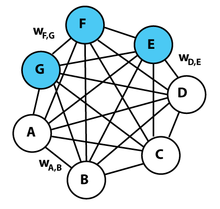
\includegraphics[height=2in]{BM.png}
					    \caption{A Boltzmann Machine}
			\end{figure}
   		\end{center}
	}


	\frame{\frametitle{A Simplified Boltzmann Machine As A Learning Module} 
		The issue with Boltzmann Machines: Learning takes a long time
		
		\begin{block}{A Solution}
			We can restrict the topology of the network to speed training, and create useful properties of the machine. Represent the machine as a bipartite graph, where the visible layer and hidden layer only connect between each other, and never to themselves.
		\end{block}
	}

	\frame{\frametitle{A Simplified Boltzmann Machine As A Learning Module} 

			\begin{figure}
				
				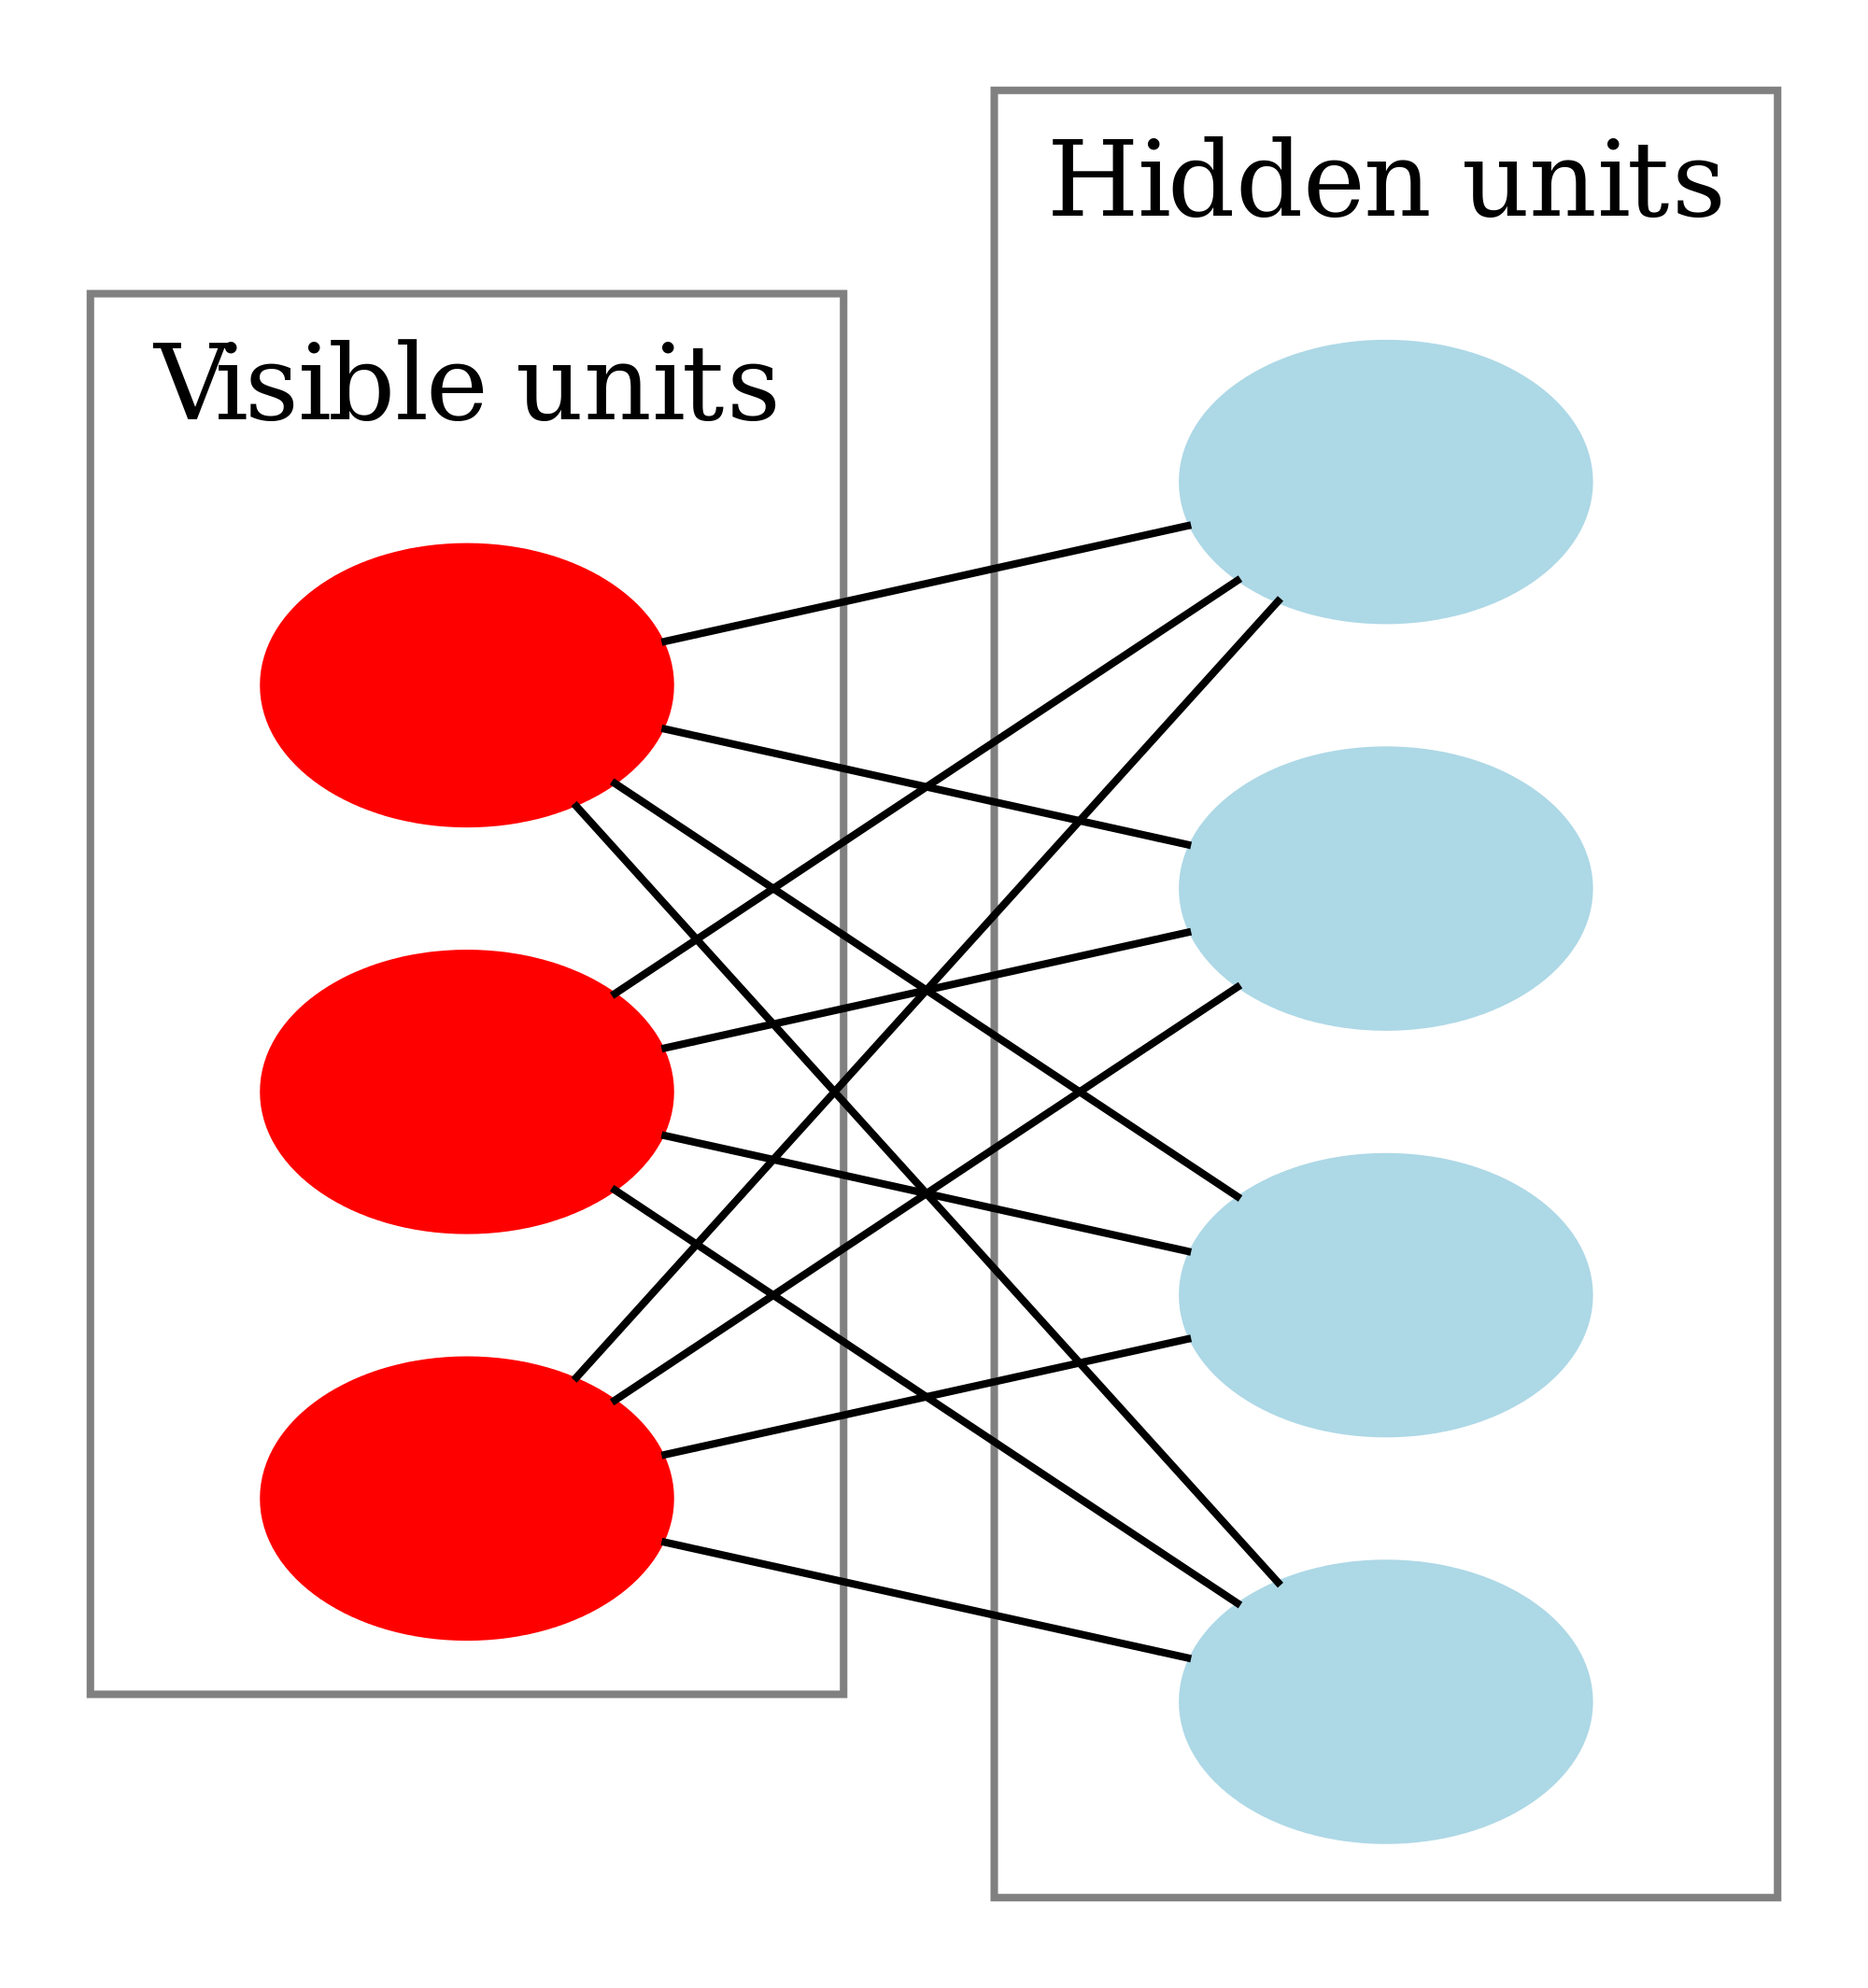
\includegraphics[height=2in]{rbm.png}
				\caption{A Restricted Boltzmann Machine}
			\end{figure}
	}

	\frame{\frametitle{A Simplified Boltzmann Machine As A Learning Module} 
		\begin{itemize}
			
			\item One layer of hidden units, meaning one layer of features?
			\item No connections between hidden units, visible restriction may be lifted later.
			
		\end{itemize}
		
				\begin{block}{Independence of Hidden States}
					The hidden units are independent given the visible states, so sampling the posterior over "causes" of data vector are quick and unbiased.
				\end{block}

	}



	\frame{\frametitle{The Energy Function} 
		\begin{itemize}
		\item RBMs are governed by an energy function based on natural systems. Energy is lost from a system as it seeks a stable state.
		\item	The energy is determined by the weights and biases.
		\item	The energy of a connection from visible to hidden units determines the probability the network will
		choose a particular configuration.
		
		\item	The weights determine the energies linearly. The probabilities are an exponential function of the weights. Thus the log-probabilities are a linear function of the weights.
				\end{itemize}
	}
	

	\frame{\frametitle{The Maximum Likelihood Learning Algorithm} 
					\begin{figure}						
						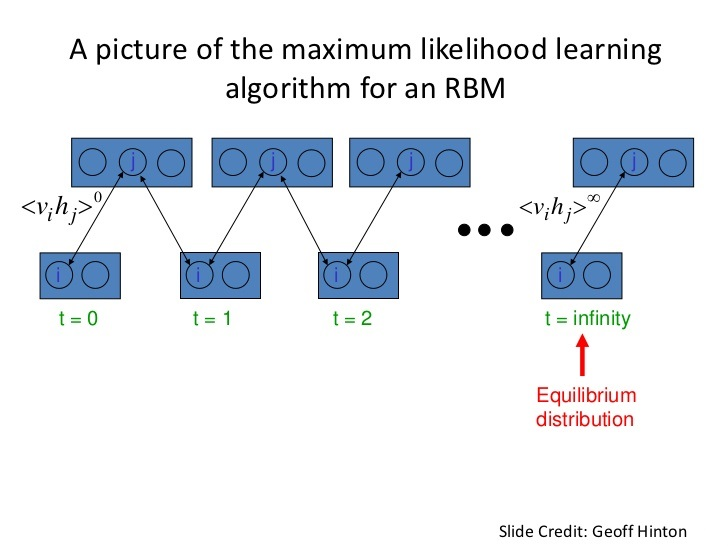
\includegraphics[height=2in]{maxlike.jpg}
						\hspace*{15pt}\hbox{\scriptsize Credit:\thinspace{\small\itshape Geoffrey Hinton }}
					\end{figure}
				\begin{equation}
					$\dfrac{\delta\log P(v)}{\delta w_{ij}} = <v_{i}h_{j}>^{0} - <v_{i}h_{j}>^{\infty}$
				\end{equation}
	}
	


	\frame{\frametitle{Hinton's Improved Algorithm} 
		\begin{itemize}
			\item Start with a training vector on the visible units.
			\item Update the hidden units, Increment weights from an active pixel to an active feature.
			\item Create a reconstruction on the visible units.
			\item Update the hidden units again Decrement weights from an active pixel to an active feature.
		\end{itemize}
		
		\begin{equation}
					$ \Delta w_{ij} = \epsilon(<v_{i}h_{j}>^{0} - <v_{i}h_{j}>^{1})$
		\end{equation}

	}
	
	
	\frame{\frametitle{An Example Using Images Of The Digit 2} 
			\begin{itemize}
				\item Data: 16 by 16 pixel image (256 visible nodes)
				\item 50 Binary Feature Neurons
				\item IMPORTANT: Increment connections on the data, decrement them on the reconstruction.
			\end{itemize}

	}
	
	\frame{\frametitle{The Maximum Likelihood Learning Algorithm} 
		\begin{figure}						
			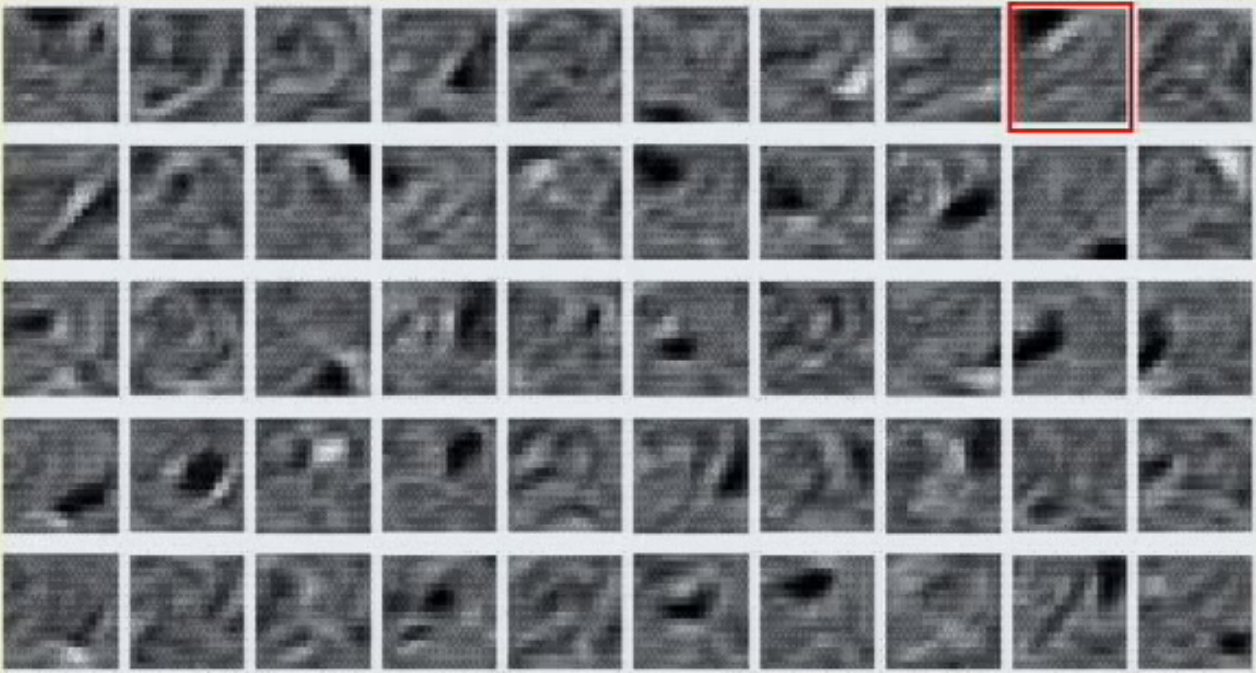
\includegraphics[height=2in]{features.png}
				\hspace*{15pt}\hbox{\scriptsize Credit:\thinspace{\small\itshape Geoffrey Hinton }}
		\end{figure}

	}
	
	

	\frame{\frametitle{Visualization Of Features On The Digit 2} 
		\begin{figure}						
			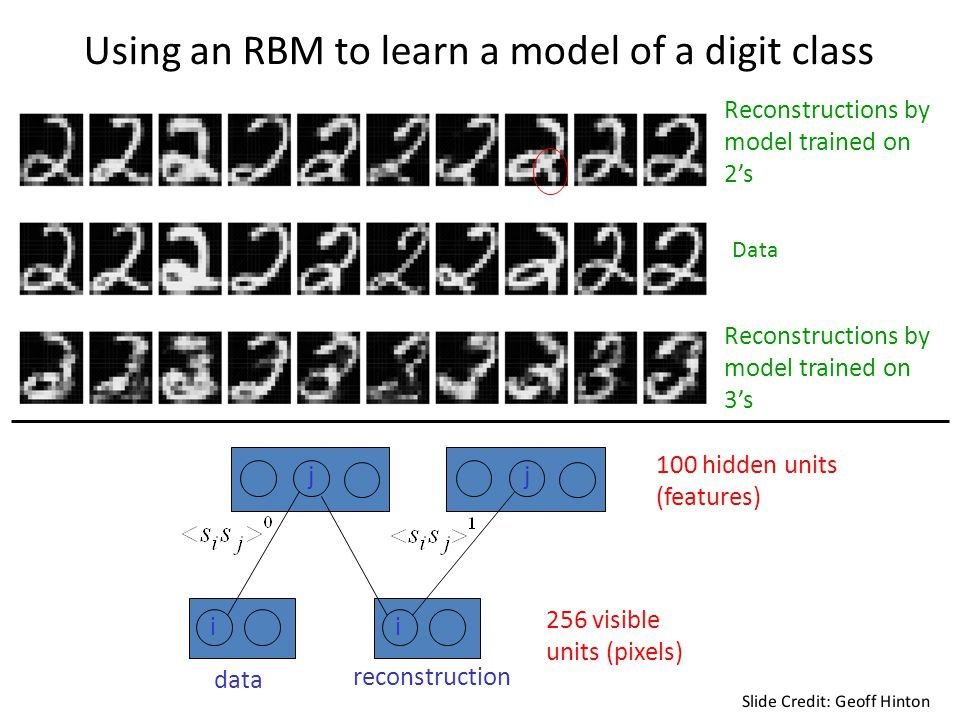
\includegraphics[height=2.5in]{slide_19.jpg}
				\hspace*{15pt}\hbox{\scriptsize Credit:\thinspace{\small\itshape Geoffrey Hinton }}
		\end{figure}
					
	}


\section{Restricted Boltzmann Machines in Deep Learning}
	\frame{\frametitle{Layers Of Features: Greedy Learning A Deep Network} 
		\begin{itemize}
			\item Begin by training the first layer as with a single RBM.
			\item Treat the activations of the trained features as the data vector for the next hidden layer.
			\item It can be proved that each time a layer is added, we improve our model of the training set.
			
		\end{itemize}
		\begin{block}{}
			The proof uses variational free energy, a method used in physics for analyzing complicated non-equilibrium systems.
		\end{block}
	}
	

\frame{\frametitle{An Explanation Of Greedy Learning}
	\begin{itemize}
		\item Each layer (RBM) converts its data distribution (input) into a posterior distrobution over its hidden units.
		\item Modeling made of 2 tasks
		\begin{enumerate}
			\item Learn generative weights that can convert the posterior back into data $P(v|h,W)$
			\item Learn to model the posterior distribution over the hidden units $P(h|W)$
		\end{enumerate}
		
		
	\end{itemize}

	\begin{block}{}
		Hinton calls this process "creeping parameterization"
	\end{block}
}

\frame{\frametitle{A Deep Belief Network For Digit Classification} 
		\begin{figure}						
			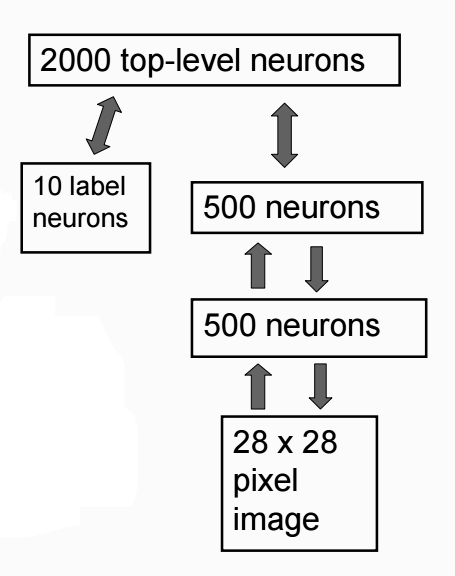
\includegraphics[height=2.5in]{dbn.png}
				\hspace*{15pt}\hbox{\scriptsize Credit:\thinspace{\small\itshape Geoffrey Hinton }}
		\end{figure}
}

\section{RBMs For Dimensionality Reduction}

\frame{\frametitle{Deep Autoencoders}
	
	\begin{block}{}
		We can communicate data into a bottleneck of RBMs to perform non-linear dimensionality reduction.
	\end{block}
	
	\begin{itemize}
		\item Optimizing deep autoencoders via backprop is very difficult (The gradient issue).
		\item A better solution
		\begin{itemize}
			\item Train the first "stack" of RBMs
			\item Then unroll them
			\item Fine tune with backprop
		\end{itemize}
	\end{itemize}

}

\frame{\frametitle{Deep Autoencoders}
	
		\begin{figure}						
			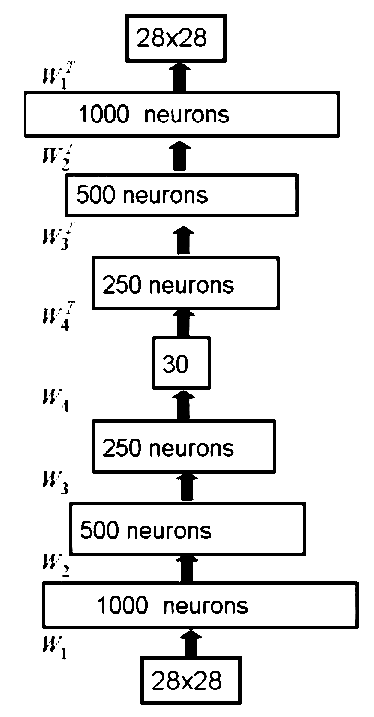
\includegraphics[height=2in]{dpca935_bw.png}
					\hspace*{15pt}\hbox{\scriptsize Credit:\thinspace{\small\itshape Geoffrey Hinton }}
			\caption{A deep autoencoder}
		\end{figure}
	
}

\frame{\frametitle{Deep Autoencoders}
	\begin{block}{PCA vs Deep Autoencoder}
		The top row is the original data, followed by the autoencoder and finally PCA.
	\end{block}
	\begin{figure}						
		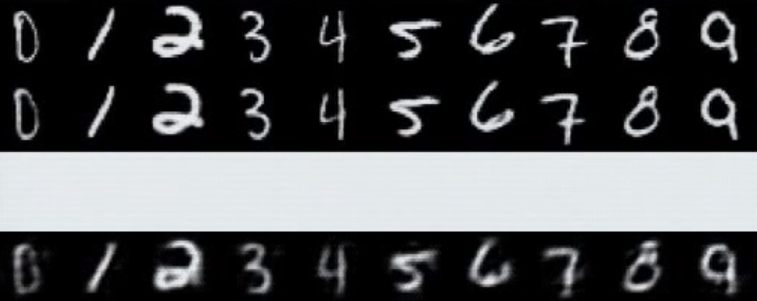
\includegraphics[height=1in]{dpca_res.png}
		\hspace*{15pt}\hbox{\scriptsize Credit:\thinspace{\small\itshape Geoffrey Hinton }}
	\end{figure}
	
}

\section{Conclusion}

\frame{\frametitle{Summary}
	\begin{itemize}
		\item Restricted Boltzmann Machines allow the extraction of features from a probability distribution without any labeled data
		\item The Restriction on network topology reduces computation time and allows the prior distribution to be sampled without bias
		\item Many layers of RBMs can be linked to create a Deep Belief Network, for generation or classification, without any labeled data
		\item These principals can be applied as non-linear dimensionality reduction
	\end{itemize}
}




\section{Sources}

\frame{begin{frame}[allowframebreaks]
	\frametitle<presentation>{Further Reading}    
	\begin{thebibliography}{10}    
		\beamertemplatebookbibitems
		\bibitem{	Hinton2002}
		Hinton, G.E.
		\newblock {\em Training products of experts by minimizing contrastive divergence.
			Neural Computation 14, 1771–1800 (2002)}.
		\newblock Klein-Verlag, 1990.
		\beamertemplatearticlebibitems
		\bibitem{Norouzi2006}
		Norouzi, M.
		
		\newblock {\em Convolutional Restricted Boltzmann Machines For Feature Learning. Simon Fraser University, (2009)}
		
		\beamertemplatearticlebibitems
		\bibitem{Fischer2013}
		Fischer, A
		
		\newblock {\em An Introduction to Restricted Boltzmann Machines (2013)}
	\end{thebibliography}
}

\end{document}
